
TDOA (Time Difference of Arrival) method, as one of the classic SSL (Sound Source Localization) method, performs excellently in environments with low noise and low reverberation. Its principle involves triangulating the position based on the time differences in the arrival of signals.

Assuming a system composed of two microphones located at coordinates \((x_1, y_1)\) and \((x_2, y_2)\), with the speed of sound in the current environment being \(c\). When a sound is emitted from the source and received by the two microphones, the TDOA value obtained is \(t_{12}\). Multiplying the TDOA value by \(c\) gives the distance difference between the sound source and the two microphones. Based on this, we can solve for the coordinates of the sound source:
\[
\sqrt{(x-x_{1})^{2}+(y-y_{1})^{2}}-\sqrt{(x-x_{2})^{2}+(y-y_{2})^{2}}=c*t_{1-2}
\]
Solving this equation, the result is a hyperbola representing all possible locations of the sound source under TDOA. By adding a third point, the intersection of two hyperbolas allows us to accurately determine the position of the sound source.\\
\begin{figure}[H]
    \centering
    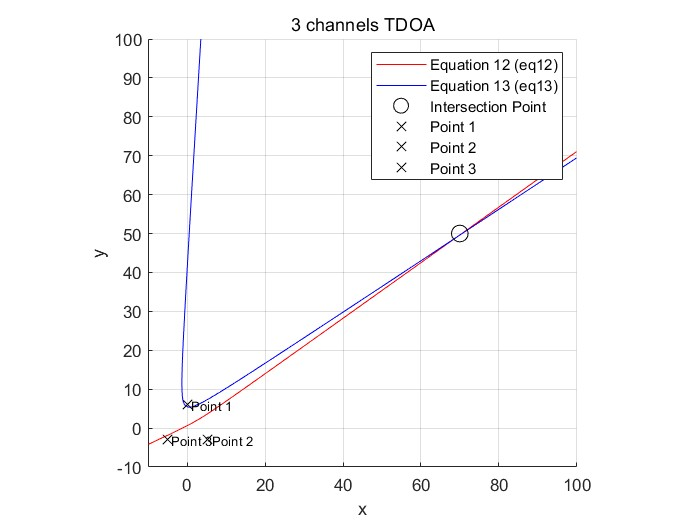
\includegraphics[width=0.7\linewidth]{figures/3_Channels.jpg}
    \caption{3-Channel TDOA Localization Schematic Diagram}
\end{figure}
Generally, there are two ways to obtain TDOA values: 

The first method involves subtracting the time of arrival (TOA) at each receiver. The limitation of this approach is that acquiring TOA requires strict synchronization between the signal source and the receivers. Therefore, this method is not suitable for locating randomly occurring signal sources in an environment.

The second method involves performing correlation calculations on the signals received by two receivers to obtain the TDOA value. This method does not require time synchronization between the sound source and the receivers, making it applicable in a wider range of scenarios and suitable for processing sporadic sound information in the environment. Therefore, this project employs the second method to solve for the TDOA value. 

In our project, the specific methods and principles are as follows:
\begin{enumerate}
    \item Collecting the sound pressure signals from each receivers while ensure all the receivers are time-synchronized. The signals are represented as the following matrix:
    \[
        \mathbf{S} = 
        \begin{bmatrix}
            s_1(t)\\
            s_2(t)\\
            \vdots\\
            s_6(t)\\
        \end{bmatrix}
    \]
    \(s_1\) to \(s_6\) is the signals of 6 channels (according to \textit{ The Geometry of the Hexagonal Microphone Array}, corresponding to M1 through M6).
    \item The project team divides the microphone array into 2 groups: M1 M3 M5 and M2 M4 M6. These two sets of signals, based on M1 and M2, are used for GCC (Generalized Cross-Correlation) calculation. The detail calculations are as following:
    
\end{enumerate}

